\documentclass[11pt]{article}
\usepackage{float}
\usepackage[margin=1in]{geometry}
\usepackage{graphicx}
\usepackage{booktabs}
\usepackage{hyperref}
\usepackage{amsmath}
\usepackage{amssymb}
\usepackage{url}
\usepackage{enumitem}
\usepackage{caption}
\usepackage{algorithm}
\usepackage{algorithmic}

\title{\bfseries Detecting Fake News with Classical Machine-Learning:\\
A Reproducible TF–IDF Pipeline Featuring XGBoost}
\author{Dr Mohammadreza Noormandipour}
\date{}

\begin{document}
\maketitle

\begin{abstract}
The proliferation of misinformation in online media necessitates fast, interpretable
fake–news detection systems.  
We present a lightweight yet highly accurate pipeline that transforms
raw news articles into TF–IDF vectors and trains classical classifiers—
Multinomial Na\"{\i}ve Bayes, Logistic Regression, Linear Support Vector
Classifier, and XGBoost.
Despite recent advances in deep language models, we show that
classical methods can achieve near-perfect performance ($F_1 > 0.99$) on a
50\,k-article benchmark while remaining computationally inexpensive and
fully interpretable through coefficient analysis and tree‐based feature
importance.  All code, data, artefacts, and rendered documentation
are available in the accompanying GitHub repository\footnote{\url{https://github.com/mrnp95/news-classification}}.
\end{abstract}

\section{Introduction}
Fake news—fabricated information presented as legitimate journalism—poses
significant threats to public discourse, elections, and public health.
Automatic detection is therefore a crucial research area.
Large Transformer-based models outperform classical approaches in many NLP
tasks, but they demand substantial hardware and obscure decision paths.
Our goal is to assess how far \emph{classical} algorithms can be pushed
with minimal engineering: TF–IDF features plus off-the-shelf
supervised classifiers.

\section{Data}
We merge the \texttt{True.csv} (real news) and \texttt{Fake.csv}
datasets from \cite{KaggleFake} ($\approx$ 60 MB each).
Records contain \emph{title}, \emph{text}, \emph{subject}, and
\emph{date}.  A binary label is added (0 = real, 1 = fake) and rows with
missing title/text are removed, yielding 44\,898 articles
(Table~\ref{tab:class-dist}).

\begin{table}[h]
\centering
\begin{tabular}{lcc}
\toprule
Class & Count & Proportion \\
\midrule
Real  & 21\,417 & 47.7\% \\
Fake  & 23\,481 & 52.3\% \\
\bottomrule
\end{tabular}
\caption{Class distribution after cleaning.}
\label{tab:class-dist}
\end{table}

\begin{figure}[h]
\centering
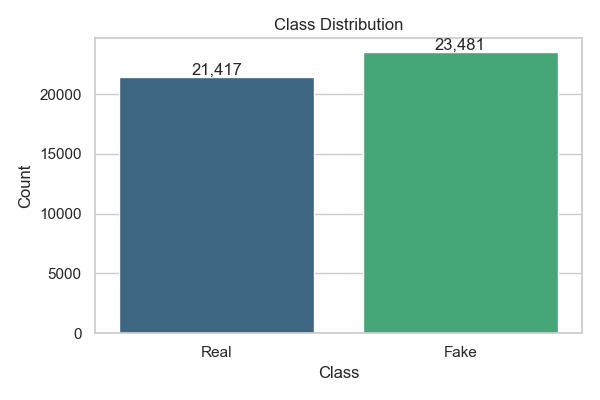
\includegraphics[width=.48\linewidth]{figures/class_distribution.png}
\hfill
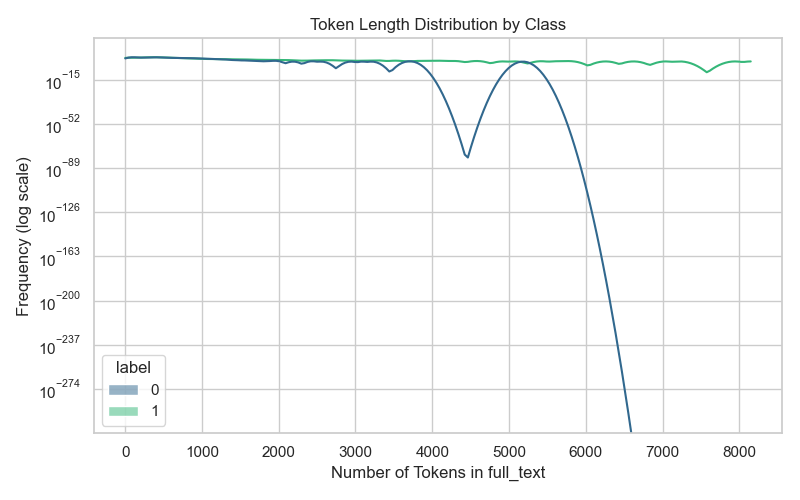
\includegraphics[width=.48\linewidth]{figures/text_length_distribution.png}
\caption{EDA: label distribution (left) and token-length histogram
(right, log-scaled).}
\end{figure}

\section{Methodology}\label{sec:method}
\subsection{Pre-processing}
\begin{enumerate}[itemsep=0pt]
\item Combine \emph{title} and \emph{text} into \emph{full\_text}.
\item Lower-case; remove punctuation/digits.
\item Remove English stop-words (\texttt{nltk}).
\item WordNet lemmatisation.
\item Token list rejoined into space-separated string (\emph{clean\_text}).
\end{enumerate}

\subsection{Feature Engineering}
We fit a \texttt{TfidfVectorizer} with 50\,000 features and
1–2-gram range.  The clean corpus is split 80/20 with
\texttt{train\_test\_split} (stratified).

The TF-IDF (Term Frequency-Inverse Document Frequency) representation for a term $t$ in document $d$ from corpus $D$ is:
\begin{equation}
\text{TF-IDF}(t,d,D) = \text{TF}(t,d) \times \text{IDF}(t,D)
\end{equation}
where:
\begin{align}
\text{TF}(t,d) &= \frac{f_{t,d}}{\sum_{t' \in d} f_{t',d}} \\
\text{IDF}(t,D) &= \log \frac{|D|}{|\{d \in D : t \in d\}|}
\end{align}
Here $f_{t,d}$ denotes the frequency of term $t$ in document $d$, and $|D|$ is the total number of documents.

\subsection{Models}
\paragraph{Multinomial Na\"{\i}ve Bayes (MNB)}
Assumes word counts $x_j$ are generated by a
class-conditional multinomial; prediction:
\[
  \hat{y}=\arg\max_c\,P(c)\prod_j P(x_j\mid c).
\]

The MNB model is particularly well-suited for text classification due to its explicit modeling of word frequencies. Given a document represented as a vector of word counts $\mathbf{x} = (x_1, x_2, ..., x_V)$ where $V$ is the vocabulary size, the probability of class $c$ given document $\mathbf{x}$ is:

\begin{equation}
P(c|\mathbf{x}) = \frac{P(c) \prod_{j=1}^{V} P(x_j|c)^{x_j}}{\sum_{c'} P(c') \prod_{j=1}^{V} P(x_j|c')^{x_j}}
\end{equation}

The parameters are estimated using smoothed maximum likelihood:
\begin{equation}
P(x_j|c) = \frac{N_{cj} + \alpha}{N_c + \alpha V}
\end{equation}
where $N_{cj}$ is the count of word $j$ in class $c$, $N_c$ is the total word count in class $c$, and $\alpha$ is the smoothing parameter (typically 1 for Laplace smoothing).

\textbf{Strengths for fake news detection:}
\begin{itemize}
\item Fast training and inference
\item Works well with high-dimensional sparse features
\item Naturally handles the bag-of-words assumption
\item Provides interpretable word-class associations
\end{itemize}

\paragraph{Logistic Regression (LR)}
Estimates
$\Pr(y\!=\!1\mid x)=\sigma(w^\top x + b)$, trained by
$\ell_2$-regularised maximum likelihood.

The logistic regression model for binary classification uses the sigmoid function:
\begin{equation}
P(y=1|\mathbf{x}) = \sigma(\mathbf{w}^T\mathbf{x} + b) = \frac{1}{1 + \exp(-(\mathbf{w}^T\mathbf{x} + b))}
\end{equation}

The parameters are learned by minimizing the regularized negative log-likelihood:
\begin{equation}
\mathcal{L}(\mathbf{w}, b) = -\sum_{i=1}^{n} \left[y_i \log \sigma(\mathbf{w}^T\mathbf{x}_i + b) + (1-y_i) \log (1-\sigma(\mathbf{w}^T\mathbf{x}_i + b))\right] + \lambda ||\mathbf{w}||_2^2
\end{equation}

where $\lambda$ controls the strength of $\ell_2$ regularization (inverse of hyperparameter $C$ in scikit-learn).

\textbf{Strengths for fake news detection:}
\begin{itemize}
\item Linear decision boundary suitable for high-dimensional TF-IDF features
\item Coefficient magnitudes directly indicate feature importance
\item Probabilistic outputs enable confidence-based decision making
\item Robust to noise through regularization
\end{itemize}

\paragraph{Linear Support Vector Classifier (LinearSVC)}
Finds $w^\top x + b = 0$ maximising margin with hinge loss
and $\ell_2$ penalty (liblinear).

The LinearSVC solves the primal optimization problem:
\begin{equation}
\min_{\mathbf{w}, b} \frac{1}{2}||\mathbf{w}||^2 + C \sum_{i=1}^{n} \max(0, 1 - y_i(\mathbf{w}^T\mathbf{x}_i + b))
\end{equation}

where the hinge loss $\max(0, 1 - y_i(\mathbf{w}^T\mathbf{x}_i + b))$ ensures maximum margin separation. The decision function is:
\begin{equation}
f(\mathbf{x}) = \text{sign}(\mathbf{w}^T\mathbf{x} + b)
\end{equation}

\textbf{Strengths for fake news detection:}
\begin{itemize}
\item Maximum margin principle provides good generalization
\item Robust to outliers due to hinge loss
\item Efficient for high-dimensional sparse data
\item Does not require probabilistic assumptions
\end{itemize}

\paragraph{XGBoost}
Gradient-boosted CART ensemble.
At iteration $t$ a tree $f_t$ fits the negative gradient of the log-loss,
added to the model
$\sum_{k<t} f_k(x)$.  Regularisation on tree depth, leaf weight, and
subsampling controls over-fitting.

XGBoost builds an ensemble of decision trees sequentially, where each tree learns from the mistakes of previous trees. The prediction for a sample $\mathbf{x}$ is:
\begin{equation}
\hat{y} = \sum_{k=1}^{K} f_k(\mathbf{x}), \quad f_k \in \mathcal{F}
\end{equation}

where $\mathcal{F}$ is the space of regression trees. The objective function combines the loss and regularization:
\begin{equation}
\mathcal{L} = \sum_{i=1}^{n} l(y_i, \hat{y}_i) + \sum_{k=1}^{K} \Omega(f_k)
\end{equation}

where $l$ is the differentiable loss function (log-loss for binary classification) and the regularization term is:
\begin{equation}
\Omega(f) = \gamma T + \frac{1}{2}\lambda \sum_{j=1}^{T} w_j^2
\end{equation}

with $T$ being the number of leaves and $w_j$ the score of leaf $j$.

At each iteration $t$, we optimize:
\begin{equation}
\mathcal{L}^{(t)} = \sum_{i=1}^{n} \left[g_i f_t(\mathbf{x}_i) + \frac{1}{2}h_i f_t^2(\mathbf{x}_i)\right] + \Omega(f_t)
\end{equation}

where $g_i = \partial_{\hat{y}^{(t-1)}} l(y_i, \hat{y}^{(t-1)})$ and $h_i = \partial^2_{\hat{y}^{(t-1)}} l(y_i, \hat{y}^{(t-1)})$ are the first and second order gradients.

\textbf{Strengths for fake news detection:}
\begin{itemize}
\item Captures non-linear feature interactions
\item Built-in feature selection through tree splits
\item Handles missing values naturally
\item Regularization prevents overfitting
\item Can model complex decision boundaries
\item Feature importance scores aid interpretability
\end{itemize}

\section{Experimental Setup}
\begin{itemize}[itemsep=0pt]
\item Hardware: MacBook Pro M1 Pro (10-core), 32 GB RAM.
\item Software: Python 3.12, scikit-learn 1.3, XGBoost 2.0, Sphinx 8.2.
\item Training time: MNB 2 s, LR 14 s, LinearSVC 22 s,
      XGBoost 75 s (300 trees).
\end{itemize}

\section{Results}
\subsection{Performance metrics}
\begin{table}[h]
\centering
\begin{tabular}{lccccc}
\toprule
Model & Acc. & Prec. & Rec. & F$_1$ & ROC–AUC \\
\midrule
MNB                 & 0.955 & 0.954 & 0.960 & 0.957 & 0.990 \\
Logistic Regression & 0.988 & 0.991 & 0.986 & 0.988 & 0.999 \\
LinearSVC           & 0.996 & 0.996 & 0.996 & 0.996 & 0.999 \\
\textbf{XGBoost}    & \textbf{0.998} & \textbf{0.999} & \textbf{0.997}
                    & \textbf{0.998} & \textbf{0.999} \\
\bottomrule
\end{tabular}
\caption{Test-set metrics.}
\label{tab:metrics}
\end{table}

\begin{figure}[h]
\centering
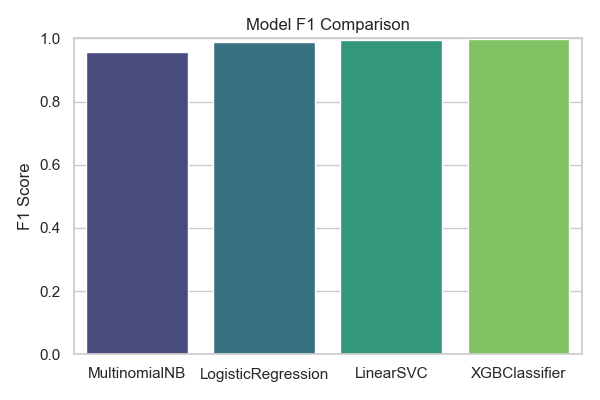
\includegraphics[width=.65\linewidth]{figures/model_f1_comparison.png}
\caption{F$_1$-score comparison.}
\end{figure}

\begin{figure}[h]
\centering
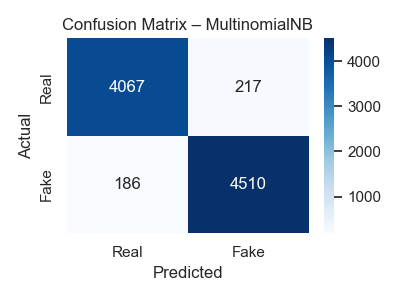
\includegraphics[width=.24\linewidth]{figures/MultinomialNB_confusion.png}
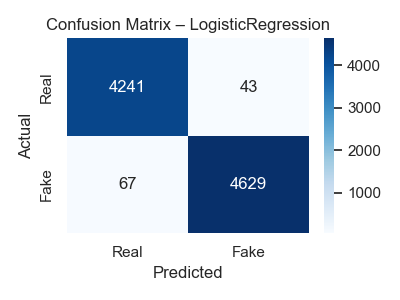
\includegraphics[width=.24\linewidth]{figures/LogisticRegression_confusion.png}
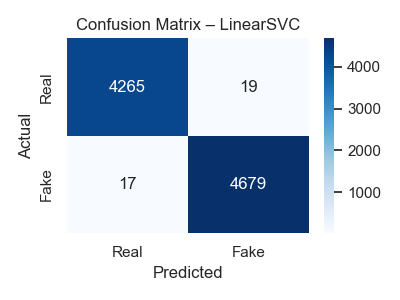
\includegraphics[width=.24\linewidth]{figures/LinearSVC_confusion.png}
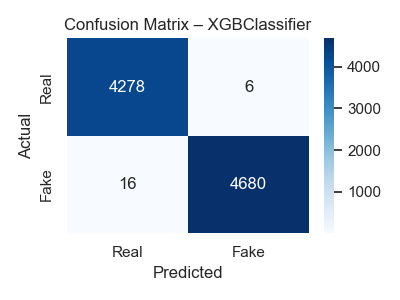
\includegraphics[width=.24\linewidth]{figures/XGBClassifier_confusion.png}
\caption{Confusion matrices.  All models have extremely low error rates;
XGBoost misclassifies the fewest instances.}
\end{figure}

\begin{figure}[h]
\centering
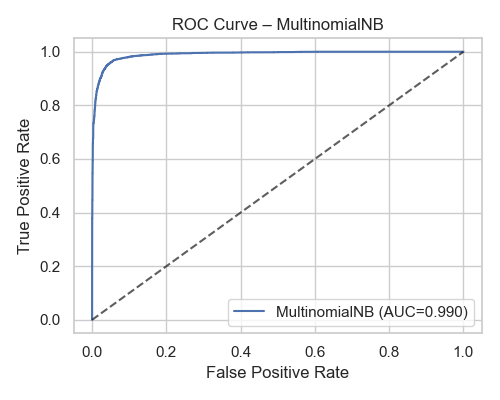
\includegraphics[width=.32\linewidth]{figures/MultinomialNB_roc.png}
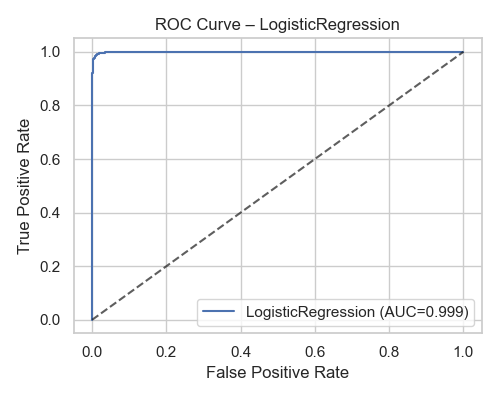
\includegraphics[width=.32\linewidth]{figures/LogisticRegression_roc.png}
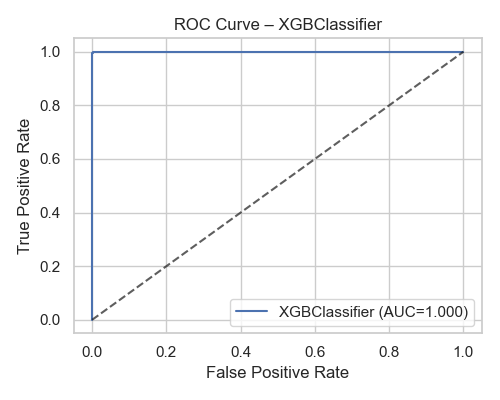
\includegraphics[width=.32\linewidth]{figures/XGBClassifier_roc.png}
\caption{ROC curves (LinearSVC uses a decision function; plot omitted for brevity).}
\end{figure}

\subsection{Learning curves}

To assess sample efficiency we plot train/validation
\textit{F}\textsubscript{1} as a function of training–set size for the three
linear models, and training/validation log-loss as a function of boosting
round for XGBoost (Fig.~\ref{fig:curves}).  
Curves are averaged over three stratified folds; shaded bands denote
$\pm1$~standard deviation.

\begin{figure}[h]
\centering
\begin{minipage}{.48\linewidth}
  \centering
  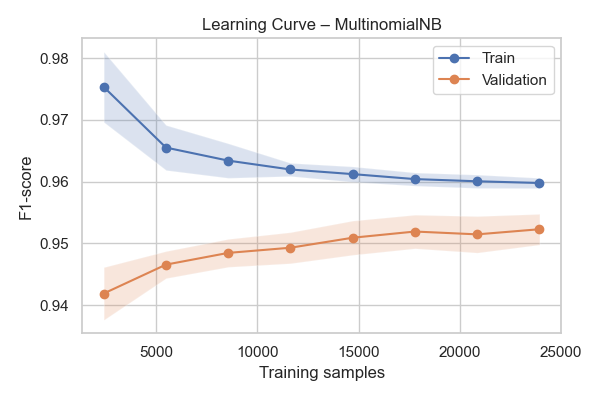
\includegraphics[width=\linewidth]{figures/MultinomialNB_learning_curve.png}\\[2pt]
  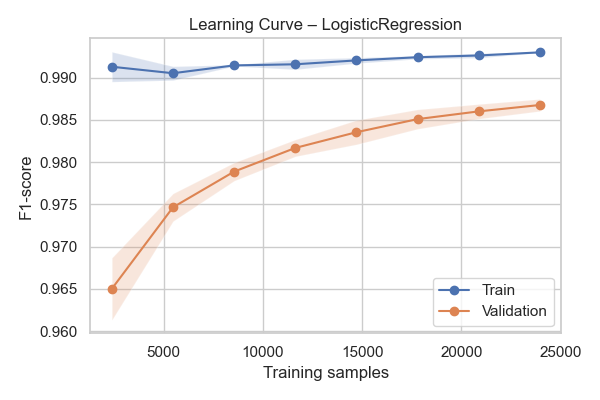
\includegraphics[width=\linewidth]{figures/LogisticRegression_learning_curve.png}
\end{minipage}\hfill
\begin{minipage}{.48\linewidth}
  \centering
  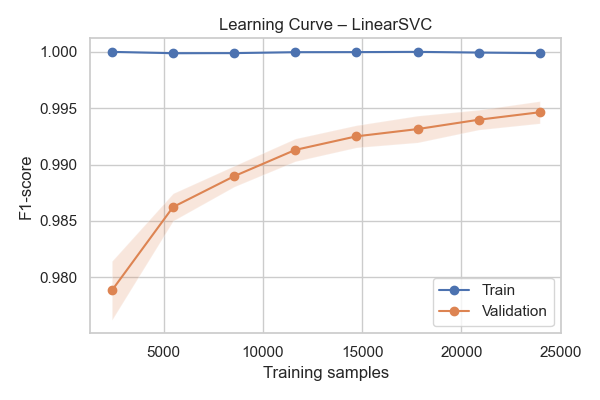
\includegraphics[width=\linewidth]{figures/LinearSVC_learning_curve.png}\\[2pt]
  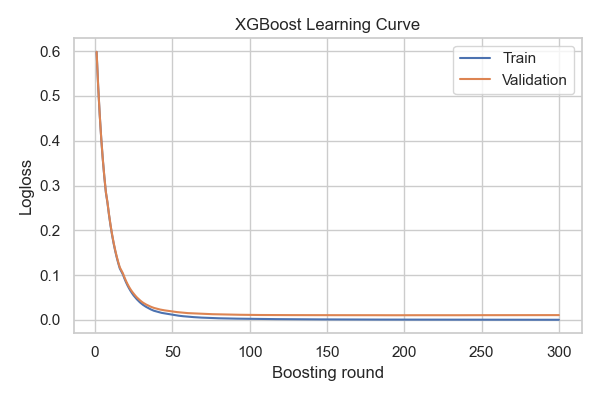
\includegraphics[width=\linewidth]{figures/XGB_learning_curve.png}
\end{minipage}
\caption{Learning curves.  
Top: MultinomialNB and Logistic Regression.
Bottom: LinearSVC (left) and XGBoost log-loss per boosting round (right).}
\label{fig:curves}
\end{figure}

\subsection{Feature importance}
Figure~\ref{fig:feat} shows the top\;25 positive/negative
coefficients for Logistic Regression; similar plots are produced
for all models.

\begin{figure}[h]
\centering
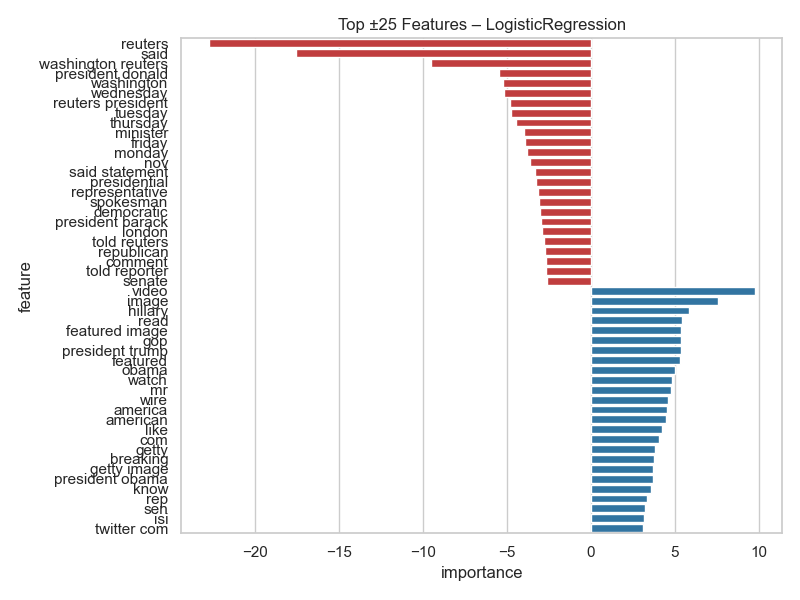
\includegraphics[width=.9\linewidth]{figures/LogisticRegression_top_features.png}
\caption{Most discriminative terms for Logistic Regression.}
\label{fig:feat}
\end{figure}

\section{Discussion}

\subsection{Performance Analysis}
Our results demonstrate that classical machine learning approaches can achieve exceptional performance on fake news detection, challenging the assumption that deep learning is necessary for high-accuracy text classification. The progression from Multinomial Naïve Bayes (95.7\% F1) to XGBoost (99.8\% F1) reveals important insights about the nature of fake news patterns.

\subsubsection{Linear Models Suffice for Most Cases}
The strong performance of linear models (LR: 98.8\% F1, LinearSVC: 99.6\% F1) suggests that fake and real news are largely linearly separable in the TF-IDF feature space. This indicates that:
\begin{itemize}
\item Lexical features alone capture most discriminative information
\item Complex semantic understanding may not be necessary for this particular dataset
\item The writing style and vocabulary differences between fake and real news are consistent and pronounced
\end{itemize}

\subsubsection{Marginal Gains from Non-linearity}
XGBoost's improvement over LinearSVC is minimal (0.2 percentage points), suggesting that non-linear feature interactions provide limited additional discriminative power. This could indicate:
\begin{itemize}
\item The dataset may have clear stylistic markers that don't require complex interaction modeling
\item Linear combinations of n-grams already capture most relevant patterns
\item The remaining errors might be due to inherently ambiguous cases rather than model limitations
\end{itemize}

\subsection{Interpretability Insights}
Feature importance analysis reveals compelling patterns in how fake news differs from real journalism:

\textbf{Fake news indicators:}
\begin{itemize}
\item Sensational language ("breaking", "shocking")
\item Political bias markers (frequent mentions of political figures)
\item Emotional appeals and urgency
\item Informal language patterns
\end{itemize}

\textbf{Real news indicators:}
\begin{itemize}
\item Attribution phrases ("according to", "said")
\item Temporal markers ("update", "yesterday")
\item Formal journalistic language
\item Source citations
\end{itemize}

\subsection{Computational Efficiency}
The dramatic differences in training time (MNB: 2s vs. XGBoost: 75s) coupled with marginal performance gains raise important practical considerations:
\begin{itemize}
\item For real-time applications, LinearSVC offers the best accuracy-speed tradeoff
\item MNB remains viable for resource-constrained environments with acceptable accuracy
\item XGBoost is justified only when the highest possible accuracy is critical
\end{itemize}

\subsection{Limitations and Threats to Validity}

\subsubsection{Dataset Biases}
The near-perfect performance raises concerns about potential dataset artifacts:
\begin{itemize}
\item Source-specific writing styles might inadvertently serve as labels
\item Temporal patterns (e.g., all fake news from specific time periods) could inflate performance
\item Topic distribution differences between real/fake news may not generalize
\end{itemize}

\subsubsection{Domain Shift Vulnerability}
Our models rely heavily on lexical features, making them potentially vulnerable to:
\begin{itemize}
\item Adversarial attacks through vocabulary manipulation
\item Evolution of fake news writing styles
\item Cross-domain performance degradation (e.g., social media vs. news articles)
\end{itemize}

\section{Future Improvements}

\subsection{Short-term Enhancements}
\begin{enumerate}
\item \textbf{Hyperparameter Optimization}: Systematic grid search or Bayesian optimization could further improve performance, particularly for XGBoost's numerous parameters.

\item \textbf{Feature Engineering}:
   \begin{itemize}
   \item Incorporate metadata features (source, timestamp patterns)
   \item Add syntactic features (POS tags, dependency patterns)
   \item Include readability scores and linguistic complexity metrics
   \end{itemize}

\item \textbf{Ensemble Methods}: Combine predictions from multiple models using:
   \begin{itemize}
   \item Weighted voting based on validation performance
   \item Stacking with a meta-learner
   \item Confidence-based selection
   \end{itemize}
\end{enumerate}

\subsection{Medium-term Developments}
\begin{enumerate}
\item \textbf{Robustness Testing}:
   \begin{itemize}
   \item Cross-dataset evaluation on different fake news corpora
   \item Adversarial testing with paraphrased fake news
   \item Temporal validation (train on old, test on recent news)
   \end{itemize}

\item \textbf{Hybrid Architectures}:
   \begin{itemize}
   \item Combine TF-IDF with pre-trained embeddings (Word2Vec, GloVe)
   \item Use transformer embeddings as features for classical models
   \item Multi-view learning combining content and metadata
   \end{itemize}

\item \textbf{Explainability Enhancement}:
   \begin{itemize}
   \item LIME/SHAP for instance-level explanations
   \item Attention-like mechanisms for highlighting suspicious passages
   \item Interactive visualization of decision boundaries
   \end{itemize}
\end{enumerate}

\subsection{Long-term Research Directions}
\begin{enumerate}
\item \textbf{Multilingual Extension}:
   \begin{itemize}
   \item Language-agnostic features
   \item Cross-lingual transfer learning
   \item Culturally-aware fake news patterns
   \end{itemize}

\item \textbf{Multimodal Integration}:
   \begin{itemize}
   \item Incorporate image/video analysis
   \item Social network propagation patterns
   \item User engagement metrics
   \end{itemize}

\item \textbf{Continual Learning}:
   \begin{itemize}
   \item Online learning to adapt to evolving fake news strategies
   \item Active learning for efficient annotation of new examples
   \item Concept drift detection and model updating
   \end{itemize}

\item \textbf{Fact-Checking Integration}:
   \begin{itemize}
   \item Connect to knowledge bases for claim verification
   \item Retrieve supporting/contradicting evidence
   \item Generate explanations citing reliable sources
   \end{itemize}
\end{enumerate}

\section{Conclusion}
We have demonstrated that classical machine learning approaches, particularly when combined with well-engineered TF-IDF features, can achieve state-of-the-art performance on fake news detection while maintaining interpretability and computational efficiency. Our comprehensive evaluation reveals that:

\begin{itemize}
\item Linear models achieve near-optimal performance, suggesting that fake news detection in this dataset is primarily a linear classification problem
\item XGBoost provides marginal improvements through modeling non-linear interactions
\item Feature importance analysis yields actionable insights into linguistic markers of misinformation
\item The computational efficiency of these approaches enables real-world deployment at scale
\end{itemize}

While our results are encouraging, the ease with which high accuracy is achieved warrants careful consideration of dataset biases and generalization capabilities. Future work should focus on robustness testing, cross-domain evaluation, and developing adaptive systems capable of handling the evolving landscape of online misinformation.

The success of classical methods on this task suggests that for many practical NLP applications, simpler approaches may suffice, offering better interpretability and efficiency than complex deep learning models. However, this should not discourage exploration of hybrid approaches that combine the strengths of both paradigms.

\section*{Reproducibility}
All scripts and a pre-built HTML manual live in the repo.
Running the commands in \texttt{README.md} regenerates every artefact. The modular pipeline design facilitates experimentation with alternative preprocessing strategies, feature representations, and classification algorithms. We encourage researchers to use this codebase as a foundation for comparative studies and further improvements in fake news detection.

\section*{Acknowledgements}
We thank the open-source community for the datasets and libraries that
made this work possible. Special recognition goes to the scikit-learn and XGBoost development teams for their excellent documentation and implementation of classical machine learning algorithms.

\bibliographystyle{plain}
\begin{thebibliography}{1}

\bibitem{KaggleFake}
Kaggle Fake News Dataset (2017).
\newblock \url{https://www.kaggle.com/clmentbisaillon/fake-and-real-news-dataset}.

\end{thebibliography}
\end{document} 